% Options for packages loaded elsewhere
% Options for packages loaded elsewhere
\PassOptionsToPackage{unicode}{hyperref}
\PassOptionsToPackage{hyphens}{url}
\PassOptionsToPackage{dvipsnames,svgnames,x11names}{xcolor}
%
\documentclass[
  spanish,
  10pt,
]{article}
\usepackage{xcolor}
\usepackage{amsmath,amssymb}
\setcounter{secnumdepth}{5}
\usepackage{iftex}
\ifPDFTeX
  \usepackage[T1]{fontenc}
  \usepackage[utf8]{inputenc}
  \usepackage{textcomp} % provide euro and other symbols
\else % if luatex or xetex
  \usepackage{unicode-math} % this also loads fontspec
  \defaultfontfeatures{Scale=MatchLowercase}
  \defaultfontfeatures[\rmfamily]{Ligatures=TeX,Scale=1}
\fi
\usepackage{lmodern}
\ifPDFTeX\else
  % xetex/luatex font selection
  \setmainfont[]{Arial}
\fi
% Use upquote if available, for straight quotes in verbatim environments
\IfFileExists{upquote.sty}{\usepackage{upquote}}{}
\IfFileExists{microtype.sty}{% use microtype if available
  \usepackage[]{microtype}
  \UseMicrotypeSet[protrusion]{basicmath} % disable protrusion for tt fonts
}{}
\makeatletter
\@ifundefined{KOMAClassName}{% if non-KOMA class
  \IfFileExists{parskip.sty}{%
    \usepackage{parskip}
  }{% else
    \setlength{\parindent}{0pt}
    \setlength{\parskip}{6pt plus 2pt minus 1pt}}
}{% if KOMA class
  \KOMAoptions{parskip=half}}
\makeatother
% Make \paragraph and \subparagraph free-standing
\makeatletter
\ifx\paragraph\undefined\else
  \let\oldparagraph\paragraph
  \renewcommand{\paragraph}{
    \@ifstar
      \xxxParagraphStar
      \xxxParagraphNoStar
  }
  \newcommand{\xxxParagraphStar}[1]{\oldparagraph*{#1}\mbox{}}
  \newcommand{\xxxParagraphNoStar}[1]{\oldparagraph{#1}\mbox{}}
\fi
\ifx\subparagraph\undefined\else
  \let\oldsubparagraph\subparagraph
  \renewcommand{\subparagraph}{
    \@ifstar
      \xxxSubParagraphStar
      \xxxSubParagraphNoStar
  }
  \newcommand{\xxxSubParagraphStar}[1]{\oldsubparagraph*{#1}\mbox{}}
  \newcommand{\xxxSubParagraphNoStar}[1]{\oldsubparagraph{#1}\mbox{}}
\fi
\makeatother


\usepackage{longtable,booktabs,array}
\usepackage{calc} % for calculating minipage widths
% Correct order of tables after \paragraph or \subparagraph
\usepackage{etoolbox}
\makeatletter
\patchcmd\longtable{\par}{\if@noskipsec\mbox{}\fi\par}{}{}
\makeatother
% Allow footnotes in longtable head/foot
\IfFileExists{footnotehyper.sty}{\usepackage{footnotehyper}}{\usepackage{footnote}}
\makesavenoteenv{longtable}
\usepackage{graphicx}
\makeatletter
\newsavebox\pandoc@box
\newcommand*\pandocbounded[1]{% scales image to fit in text height/width
  \sbox\pandoc@box{#1}%
  \Gscale@div\@tempa{\textheight}{\dimexpr\ht\pandoc@box+\dp\pandoc@box\relax}%
  \Gscale@div\@tempb{\linewidth}{\wd\pandoc@box}%
  \ifdim\@tempb\p@<\@tempa\p@\let\@tempa\@tempb\fi% select the smaller of both
  \ifdim\@tempa\p@<\p@\scalebox{\@tempa}{\usebox\pandoc@box}%
  \else\usebox{\pandoc@box}%
  \fi%
}
% Set default figure placement to htbp
\def\fps@figure{htbp}
\makeatother


% definitions for citeproc citations
\NewDocumentCommand\citeproctext{}{}
\NewDocumentCommand\citeproc{mm}{%
  \begingroup\def\citeproctext{#2}\cite{#1}\endgroup}
\makeatletter
 % allow citations to break across lines
 \let\@cite@ofmt\@firstofone
 % avoid brackets around text for \cite:
 \def\@biblabel#1{}
 \def\@cite#1#2{{#1\if@tempswa , #2\fi}}
\makeatother
\newlength{\cslhangindent}
\setlength{\cslhangindent}{1.5em}
\newlength{\csllabelwidth}
\setlength{\csllabelwidth}{3em}
\newenvironment{CSLReferences}[2] % #1 hanging-indent, #2 entry-spacing
 {\begin{list}{}{%
  \setlength{\itemindent}{0pt}
  \setlength{\leftmargin}{0pt}
  \setlength{\parsep}{0pt}
  % turn on hanging indent if param 1 is 1
  \ifodd #1
   \setlength{\leftmargin}{\cslhangindent}
   \setlength{\itemindent}{-1\cslhangindent}
  \fi
  % set entry spacing
  \setlength{\itemsep}{#2\baselineskip}}}
 {\end{list}}
\usepackage{calc}
\newcommand{\CSLBlock}[1]{\hfill\break\parbox[t]{\linewidth}{\strut\ignorespaces#1\strut}}
\newcommand{\CSLLeftMargin}[1]{\parbox[t]{\csllabelwidth}{\strut#1\strut}}
\newcommand{\CSLRightInline}[1]{\parbox[t]{\linewidth - \csllabelwidth}{\strut#1\strut}}
\newcommand{\CSLIndent}[1]{\hspace{\cslhangindent}#1}

\ifLuaTeX
\usepackage[bidi=basic]{babel}
\else
\usepackage[bidi=default]{babel}
\fi
\ifPDFTeX
\else
\babelfont{rm}[]{Arial}
\fi
% get rid of language-specific shorthands (see #6817):
\let\LanguageShortHands\languageshorthands
\def\languageshorthands#1{}


\setlength{\emergencystretch}{3em} % prevent overfull lines

\providecommand{\tightlist}{%
  \setlength{\itemsep}{0pt}\setlength{\parskip}{0pt}}



 


\usepackage{booktabs}
\usepackage{longtable}
\usepackage{array}
\usepackage{multirow}
\usepackage{wrapfig}
\usepackage{float}
\usepackage{colortbl}
\usepackage{pdflscape}
\usepackage{tabu}
\usepackage{threeparttable}
\usepackage{threeparttablex}
\usepackage[normalem]{ulem}
\usepackage{makecell}
\usepackage{xcolor}
% Paquetes necesarios
\usepackage{amsmath}
\usepackage{amssymb}
\usepackage{graphicx}
\usepackage{fancyhdr}
\usepackage{geometry}
\usepackage{booktabs}
\usepackage{dcolumn}
\usepackage{array}
\newcolumntype{d}[1]{D{.}{.}{#1}}
\usepackage{float}
\usepackage{adjustbox}
\renewcommand{\normalsize}{\fontsize{10pt}{12pt}\selectfont}

% Configuración de márgenes
\geometry{
  a4paper,
  left=1.5cm,
  right=1.5cm,
  top=1.5cm,
  bottom=2.5cm,
  includeheadfoot
}

% Configuración de encabezado y pie de página
\pagestyle{fancy}
\fancyhf{} % Limpia encabezado y pie de página

% Encabezado
\lhead{
\includegraphics[height=1.5cm]{logo.png}} % Logo en el encabezado
\chead{}
\rhead{\small Econometría: Prueba 1.}

% Ajuste de separación entre encabezado y contenido
\setlength{\headheight}{2cm} % Altura del encabezado
\setlength{\headsep}{1.5cm} % Distancia entre encabezado y contenido

% Pie de página
\lfoot{}
\cfoot{\thepage} % Número de página centrado
\rfoot{}
\makeatletter
\@ifpackageloaded{caption}{}{\usepackage{caption}}
\AtBeginDocument{%
\ifdefined\contentsname
  \renewcommand*\contentsname{Tabla de contenidos}
\else
  \newcommand\contentsname{Tabla de contenidos}
\fi
\ifdefined\listfigurename
  \renewcommand*\listfigurename{Listado de Figuras}
\else
  \newcommand\listfigurename{Listado de Figuras}
\fi
\ifdefined\listtablename
  \renewcommand*\listtablename{Listado de Tablas}
\else
  \newcommand\listtablename{Listado de Tablas}
\fi
\ifdefined\figurename
  \renewcommand*\figurename{Figura}
\else
  \newcommand\figurename{Figura}
\fi
\ifdefined\tablename
  \renewcommand*\tablename{Tabla}
\else
  \newcommand\tablename{Tabla}
\fi
}
\@ifpackageloaded{float}{}{\usepackage{float}}
\floatstyle{ruled}
\@ifundefined{c@chapter}{\newfloat{codelisting}{h}{lop}}{\newfloat{codelisting}{h}{lop}[chapter]}
\floatname{codelisting}{Listado}
\newcommand*\listoflistings{\listof{codelisting}{Listado de Listados}}
\makeatother
\makeatletter
\makeatother
\makeatletter
\@ifpackageloaded{caption}{}{\usepackage{caption}}
\@ifpackageloaded{subcaption}{}{\usepackage{subcaption}}
\makeatother
\usepackage{bookmark}
\IfFileExists{xurl.sty}{\usepackage{xurl}}{} % add URL line breaks if available
\urlstyle{same}
\hypersetup{
  pdfauthor={Amaru Simón Agüero Jiménez},
  pdflang={es},
  colorlinks=true,
  linkcolor={blue},
  filecolor={Maroon},
  citecolor={Blue},
  urlcolor={Blue},
  pdfcreator={LaTeX via pandoc}}


\title{\begin{center}
  
\includegraphics[height=4cm]{logo.png} \\[1cm]
  \Large Econometría \\
\end{center}}
\usepackage{etoolbox}
\makeatletter
\providecommand{\subtitle}[1]{% add subtitle to \maketitle
  \apptocmd{\@title}{\par {\large #1 \par}}{}{}
}
\makeatother
\subtitle{Prueba 1}
\author{Amaru Simón Agüero Jiménez}
\date{2025-05-12}
\begin{document}
\maketitle

\renewcommand*\contentsname{Tabla de contenidos}
{
\hypersetup{linkcolor=}
\setcounter{tocdepth}{3}
\tableofcontents
}

\section{Paquetes de R y LaTex.}\label{paquetes-de-r-y-latex.}

\section{Caso.}\label{caso.}

Simular un proceso generador de datos para el tiempo que le toma a una
persona, negociando sobre la venta de un artículo, llegar a un acuerdo.
Nos interesa conocer los mecanismos psicológicos que operan detrás de
las decisiones cooperativas de las personas frente a conflictos de
interés (juegos de suma cero). Interpretaremos el tiempo como una medida
inversa de cooperación ---i.e., ante mayor disposición de las personas
para cooperar o compartir las ganancias de la negociación, menor debería
ser el tiempo necesario para llegar a un acuerdo.

Creemos que las personas que perciban mayores niveles de conflicto de
intereses con su contraparte implementarán tácticas de negociación menos
conciliadoras y tardarán más tiempo en llegar a un acuerdo. Esperamos,
por lo tanto, una relación directa entre el conflicto percibido y el
tiempo para alcanzar un acuerdo en la negociación. Esperamos, que esta
relación esté moderada por el rasgo de reciprocidad, donde personas con
perfiles de cooperación no-condicionales tenderían a cooperar
independientemente del conflicto percibido.

Supondremos, para este ejercicio, que el tiempo necesario para ponerse
de acuerdo (\textbf{en segundos}) es determinado \textbf{exclusivamente}
por:

\begin{enumerate}
\def\labelenumi{\arabic{enumi}.}
\item
  La percepción de conflicto de interés (\textbf{en puntaje \(z\)}), de
  los participantes en la ronda de negociación, que medimos con la
  escala psicométrica Situational Interdependence
  Scale\textsuperscript{1}.
\item
  El rasgo de reciprocidad (\textbf{dummy}), que medimos de la
  clasificación de los participantes como cooperadores
  condicionales/no-condicionales a partir de la técnica del Strategy
  Method (dCC)\textsuperscript{2}.
\item
  El rasgo de pro-socialidad (\textbf{en puntaje \(z\)}), que medimos de
  la escala Social Value Orientation (SVO)\textsuperscript{3}.
\end{enumerate}

La \textbf{variable independiente de interés} principal es la
\textbf{percepción de conflicto de interés}.

\section{Proceso generador de datos}\label{proceso-generador-de-datos}

Simular un proceso de generación de datos según lo que se especifica a
continuación. Asumir que el tiempo, la percepción de conflicto de
interés y la prosocialidad siguen distribuciones normales y que la
reciprocidad sigue una distribución de Bernoulli. Utilizar los
siguientes parámetros y semillas para generar los datos:

\begin{itemize}
\tightlist
\item
  muestra: \(n = 50\)
\item
  tiempo: \(\beta_0 = 350\), \(\beta_{conflicto} = 20\),
  \(\beta_{conflicto \times dcc} = 30\), \(\beta_{svo} = -25\)
\item
  error: \(\mathrm{E}(u) = 0\), \(\mathrm{Var}(u|x) = \sigma^2 = 80^2\),
  seed = 6
\item
  svo: \(\mu_{svo} = 0\), \(\sigma_{svo} = 1\), seed = 5
\item
  conflicto: \(\mu_{conflicto} = 0 - 0.5 \times svo\),
  \(\sigma_{conflicto} = 1\), seed = 2
\item
  dcc: \(\mu_{dcc} = 0.7\), seed = 45
\end{itemize}

\newpage

\section{Pregunta 1.}\label{pregunta-1.}

Describir el comportamiento de las variables de la muestra.

\begin{enumerate}
\def\labelenumi{(\alph{enumi})}
\tightlist
\item
  Tomar estadísticas descriptivas de las variables. Incluir, al menos,
  la media, moda, mediana y el rango intercuartílico, cuando
  corresponda.
\end{enumerate}

\begin{table}[H]
\centering
\caption{\label{tab:unnamed-chunk-3}Estadísticas descriptivas de las variables}
\centering
\begin{tabular}[t]{lll}
\toprule
Variable & Estadístico & Valor\\
\midrule
 & Media & 358.92\\
\cmidrule{2-3}
 & Desviación Estándar & 108.71\\
\cmidrule{2-3}
 & Moda & 368.77\\
\cmidrule{2-3}
 & Mediana & 359.47\\
\cmidrule{2-3}
\multirow[t]{-5}{*}{\raggedright\arraybackslash Tiempo} & IQR & 150.41\\
\cmidrule{1-3}
 & Media & 0.04\\
\cmidrule{2-3}
 & Desviación Estándar & 1.15\\
\cmidrule{2-3}
 & Moda & -0.48\\
\cmidrule{2-3}
 & Mediana & 0.09\\
\cmidrule{2-3}
\multirow[t]{-5}{*}{\raggedright\arraybackslash Conflicto} & IQR & 1.81\\
\cmidrule{1-3}
 & Media & 0.06\\
\cmidrule{2-3}
 & Desviación Estándar & 1.07\\
\cmidrule{2-3}
 & Moda & -0.84\\
\cmidrule{2-3}
 & Mediana & -0.14\\
\cmidrule{2-3}
\multirow[t]{-5}{*}{\raggedright\arraybackslash SVO} & IQR & 1.66\\
\cmidrule{1-3}
 & Frecuencia de No Cooperador Condicional & 9 (18\%)\\
\cmidrule{2-3}
\multirow[t]{-2}{*}{\raggedright\arraybackslash DCC} & Frecuencia de Cooperador Condicional & 41 (82\%)\\
\bottomrule
\end{tabular}
\end{table}

\newpage

\begin{enumerate}
\def\labelenumi{(\alph{enumi})}
\setcounter{enumi}{1}
\tightlist
\item
  Tomar gráficos de densidad y boxplot para variables continuas y
  gráfico de barras para variable categórica.
\end{enumerate}

\begin{figure}[H]

{\centering \pandocbounded{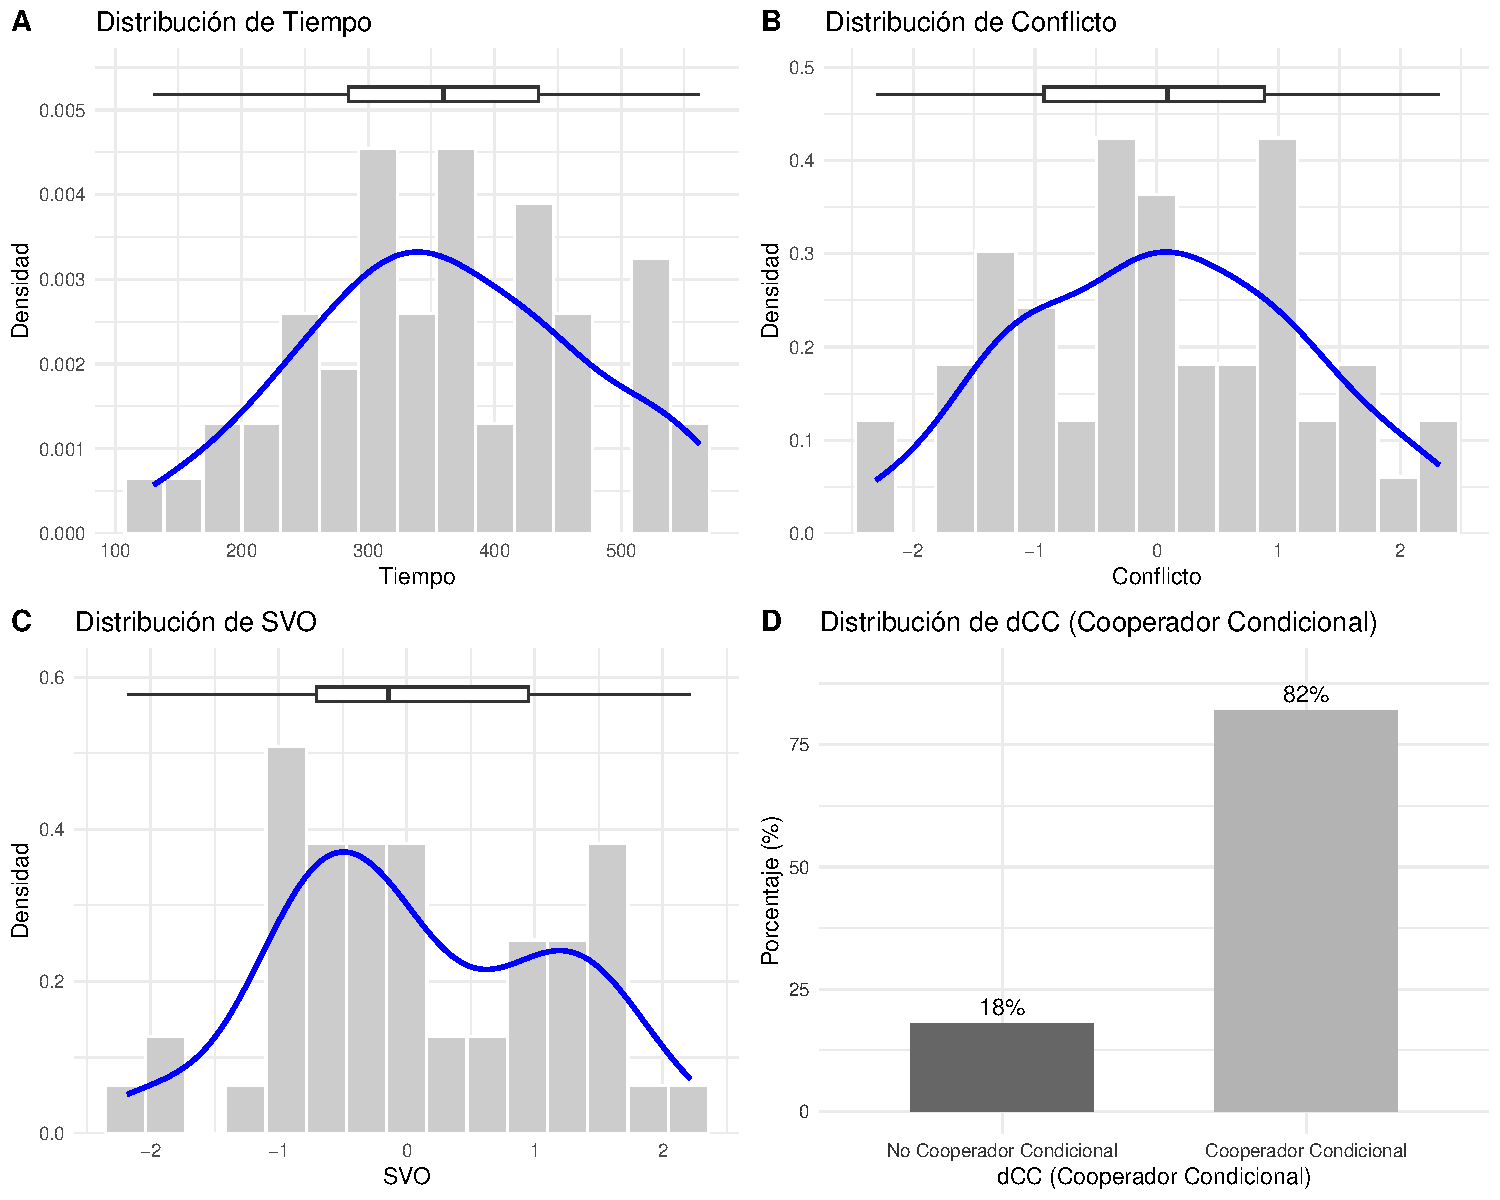
\includegraphics[keepaspectratio]{Prueba1_Amaru_Aguero_files/figure-pdf/fig1-1.pdf}}

}

\caption{Distribución de las variables continuas y categórica}

\end{figure}%

\newpage

\section{Pregunta 2.}\label{pregunta-2.}

Ajustar los 6 modelos lineales que se detallan a continuación, exportar
tabla con \texttt{stargazer()} e interpretar coeficientes y resultados
de cada modelo. Comparar y explicar diferencias entre los modelos.

\begin{enumerate}
\def\labelenumi{(\alph{enumi})}
\item
  \(tiempo \sim conflicto\)
\item
  \(tiempo \sim conflicto + svo\)
\item
  \(tiempo \sim conflicto + dcc\)
\item
  \(tiempo \sim conflicto + dcc + svo\)
\item
  \(tiempo \sim conflicto + conflicto \times dcc + dcc\)
\item
  \(tiempo \sim conflicto + conflicto \times dcc + dcc + svo\)
\end{enumerate}

\begin{table}[H] \centering 
  \caption{Resultados de los modelos lineales ajustados} 
  \label{} 
\scriptsize 
\begin{tabular}{@{\extracolsep{5pt}}lcccccc} 
\\[-1.8ex]\hline 
\hline \\[-1.8ex] 
 & \multicolumn{6}{c}{\textit{Dependent variable:}} \\ 
\cline{2-7} 
\\[-1.8ex] & \multicolumn{6}{c}{Tiempo (segundos)} \\ 
 & Modelo 1 & Modelo 2 & Modelo 3 & Modelo 4 & Modelo 5 & Modelo 6 \\ 
\hline \\[-1.8ex] 
 Conflicto & 52.72$^{***}$ (11.32) & 45.90$^{***}$ (11.30) & 54.98$^{***}$ (11.36) & 48.16$^{***}$ (11.32) & 23.65 (29.91) & 15.42 (28.86) \\ 
  SVO &  & $-$27.13$^{*}$ (12.16) &  & $-$27.02$^{*}$ (12.05) &  & $-$27.35$^{*}$ (11.99) \\ 
  dCC Si &  &  & $-$44.60 (33.68) & $-$44.12 (32.32) & $-$34.93 (34.65) & $-$34.03 (33.17) \\ 
  Conflicto $\times$ dCC Si. &  &  &  &  & 36.57 (32.32) & 38.12 (30.94) \\ 
  Constant & 356.99$^{***}$ (12.90) & 359.00$^{***}$ (12.43) & 393.48$^{***}$ (30.38) & 395.09$^{***}$ (29.17) & 383.19$^{***}$ (31.62) & 384.38$^{***}$ (30.28) \\ 
 \hline \\[-1.8ex] 
Observations & 50 & 50 & 50 & 50 & 50 & 50 \\ 
R$^{2}$ & 0.31 & 0.38 & 0.34 & 0.40 & 0.35 & 0.42 \\ 
Adjusted R$^{2}$ & 0.30 & 0.35 & 0.31 & 0.36 & 0.31 & 0.37 \\ 
Residual Std. Error & 91.16 (df = 48) & 87.60 (df = 47) & 90.45 (df = 47) & 86.81 (df = 46) & 90.18 (df = 46) & 86.32 (df = 45) \\ 
F Statistic & 21.69$^{***}$ (df = 1; 48) & 14.23$^{***}$ (df = 2; 47) & 11.89$^{***}$ (df = 2; 47) & 10.28$^{***}$ (df = 3; 46) & 8.40$^{***}$ (df = 3; 46) & 8.18$^{***}$ (df = 4; 45) \\ 
\hline 
\hline \\[-1.8ex] 
\textit{Note:}  & \multicolumn{6}{r}{$^{*}$p$<$0.05; $^{**}$p$<$0.01; $^{***}$p$<$0.001} \\ 
\end{tabular} 
\end{table}

\section{Pregunta 3.}\label{pregunta-3.}

¿Cuál modelo cree que especifica correctamente la hipótesis a probar y
por qué?

\section{Pregunta 4.}\label{pregunta-4.}

Repetir punto 2 volviendo a tomar una muestra de tiempo con
\(\beta_{conflicto \times dcc} = 10\).

\begin{table}[H] \centering 
  \caption{Resultados de los modelos lineales ajustados $\beta_{conflicto \times dcc}$ = 10} 
  \label{} 
\scriptsize 
\begin{tabular}{@{\extracolsep{5pt}}lcccccc} 
\\[-1.8ex]\hline 
\hline \\[-1.8ex] 
 & \multicolumn{6}{c}{\textit{Dependent variable:}} \\ 
\cline{2-7} 
\\[-1.8ex] & \multicolumn{6}{c}{Tiempo (segundos)} \\ 
 & Modelo 1.2 & Modelo 2.2 & Modelo 3.2 & Modelo 4.2 & Modelo 5.2 & Modelo 6.2 \\ 
\hline \\[-1.8ex] 
 Conflicto & 35.86$^{**}$ (11.16) & 29.00$^{*}$ (11.11) & 37.85$^{**}$ (11.24) & 30.99$^{**}$ (11.18) & 23.65 (29.91) & 15.42 (28.86) \\ 
  SVO &  & $-$27.29$^{*}$ (11.96) &  & $-$27.19$^{*}$ (11.90) &  & $-$27.35$^{*}$ (11.99) \\ 
  dCC Si &  &  & $-$39.31 (33.31) & $-$38.83 (31.91) & $-$34.93 (34.65) & $-$34.03 (33.17) \\ 
  Conflicto $\times$ dCC Si. &  &  &  &  & 16.57 (32.32) & 18.12 (30.94) \\ 
  Constant & 355.69$^{***}$ (12.71) & 357.71$^{***}$ (12.22) & 387.85$^{***}$ (30.05) & 389.47$^{***}$ (28.80) & 383.19$^{***}$ (31.62) & 384.38$^{***}$ (30.28) \\ 
 \hline \\[-1.8ex] 
Observations & 50 & 50 & 50 & 50 & 50 & 50 \\ 
R$^{2}$ & 0.18 & 0.26 & 0.20 & 0.28 & 0.21 & 0.29 \\ 
Adjusted R$^{2}$ & 0.16 & 0.23 & 0.17 & 0.24 & 0.15 & 0.22 \\ 
Residual Std. Error & 89.84 (df = 48) & 86.14 (df = 47) & 89.47 (df = 47) & 85.71 (df = 46) & 90.18 (df = 46) & 86.32 (df = 45) \\ 
F Statistic & 10.33$^{**}$ (df = 1; 48) & 8.22$^{***}$ (df = 2; 47) & 5.90$^{**}$ (df = 2; 47) & 6.03$^{**}$ (df = 3; 46) & 3.96$^{*}$ (df = 3; 46) & 4.54$^{**}$ (df = 4; 45) \\ 
\hline 
\hline \\[-1.8ex] 
\textit{Note:}  & \multicolumn{6}{r}{$^{*}$p$<$0.05; $^{**}$p$<$0.01; $^{***}$p$<$0.001} \\ 
\end{tabular} 
\end{table}

\section{Pregunta 5.}\label{pregunta-5.}

Repetir la simulación incrementando el tamaño de la muestra a 300
observaciones, tanto para \(\beta_{conflicto \times dcc} = 30\) como
para \(\beta_{conflicto \times dcc} = 10\) (en total en la prueba hay 4
escenarios, 2 tamaño de muestra \(\ast\) 2
\(\beta_{conflicto \times dcc}\)). Comparar con resultados anteriores y
explicar posibles causas de las diferencias.

\begin{table}[H] \centering 
  \caption{Resultados de los modelos lineales ajustados (n=300, $\beta_{conflicto \times dcc} = 30$)} 
  \label{} 
\tiny 
\begin{tabular}{@{\extracolsep{5pt}}lcccccc} 
\\[-1.8ex]\hline 
\hline \\[-1.8ex] 
 & \multicolumn{6}{c}{\textit{Dependent variable:}} \\ 
\cline{2-7} 
\\[-1.8ex] & \multicolumn{6}{c}{Tiempo (segundos)} \\ 
 & Modelo 1.3 & Modelo 2.3 & Modelo 3.3 & Modelo 4.3 & Modelo 5.3 & Modelo 6.3 \\ 
\hline \\[-1.8ex] 
 Conflicto & 52.21$^{***}$ (4.08) & 42.81$^{***}$ (4.36) & 52.18$^{***}$ (4.09) & 42.78$^{***}$ (4.37) & 31.14$^{***}$ (6.96) & 20.82$^{**}$ (6.97) \\ 
  SVO &  & $-$26.13$^{***}$ (5.27) &  & $-$26.13$^{***}$ (5.28) &  & $-$26.66$^{***}$ (5.16) \\ 
  dCC Si &  &  & $-$2.42 (10.87) & $-$2.44 (10.46) & $-$4.57 (10.66) & $-$4.66 (10.22) \\ 
  Conflicto $\times$ dCC Si &  &  &  &  & 31.47$^{***}$ (8.51) & 32.56$^{***}$ (8.17) \\ 
  Constant & 343.91$^{***}$ (4.84) & 344.69$^{***}$ (4.66) & 345.67$^{***}$ (9.27) & 346.46$^{***}$ (8.92) & 347.61$^{***}$ (9.09) & 348.49$^{***}$ (8.72) \\ 
 \hline \\[-1.8ex] 
Observations & 300 & 300 & 300 & 300 & 300 & 300 \\ 
R$^{2}$ & 0.35 & 0.40 & 0.35 & 0.40 & 0.38 & 0.43 \\ 
Adjusted R$^{2}$ & 0.35 & 0.40 & 0.35 & 0.40 & 0.38 & 0.43 \\ 
Residual Std. Error & 83.73 (df = 298) & 80.61 (df = 297) & 83.87 (df = 297) & 80.74 (df = 296) & 82.13 (df = 296) & 78.78 (df = 295) \\ 
F Statistic & 163.54$^{***}$ (df = 1; 298) & 100.51$^{***}$ (df = 2; 297) & 81.53$^{***}$ (df = 2; 297) & 66.81$^{***}$ (df = 3; 296) & 61.23$^{***}$ (df = 3; 296) & 56.61$^{***}$ (df = 4; 295) \\ 
\hline 
\hline \\[-1.8ex] 
\textit{Note:}  & \multicolumn{6}{r}{$^{*}$p$<$0.05; $^{**}$p$<$0.01; $^{***}$p$<$0.001} \\ 
\end{tabular} 
\end{table}

\begin{table}[H] \centering 
  \caption{Resultados de los modelos lineales ajustados (n=300, $\beta_{conflicto \times dcc} = 10$)} 
  \label{} 
\tiny 
\begin{tabular}{@{\extracolsep{5pt}}lcccccc} 
\\[-1.8ex]\hline 
\hline \\[-1.8ex] 
 & \multicolumn{6}{c}{\textit{Dependent variable:}} \\ 
\cline{2-7} 
\\[-1.8ex] & \multicolumn{6}{c}{Tiempo (segundos)} \\ 
 & Modelo 1.4 & Modelo 2.4 & Modelo 3.4 & Modelo 4.4 & Modelo 5.4 & Modelo 6.4 \\ 
\hline \\[-1.8ex] 
 Conflicto & 38.85$^{***}$ (4.00) & 29.33$^{***}$ (4.27) & 38.81$^{***}$ (4.01) & 29.29$^{***}$ (4.28) & 31.14$^{***}$ (6.96) & 20.82$^{**}$ (6.97) \\ 
  SVO &  & $-$26.46$^{***}$ (5.16) &  & $-$26.46$^{***}$ (5.17) &  & $-$26.66$^{***}$ (5.16) \\ 
  dCC Si &  &  & $-$3.79 (10.66) & $-$3.81 (10.23) & $-$4.57 (10.66) & $-$4.66 (10.22) \\ 
  Conflicto $\times$ dCC Si &  &  &  &  & 11.47 (8.51) & 12.56 (8.17) \\ 
  Constant & 344.15$^{***}$ (4.74) & 344.94$^{***}$ (4.56) & 346.90$^{***}$ (9.09) & 347.71$^{***}$ (8.73) & 347.61$^{***}$ (9.09) & 348.49$^{***}$ (8.72) \\ 
 \hline \\[-1.8ex] 
Observations & 300 & 300 & 300 & 300 & 300 & 300 \\ 
R$^{2}$ & 0.24 & 0.30 & 0.24 & 0.30 & 0.24 & 0.31 \\ 
Adjusted R$^{2}$ & 0.24 & 0.30 & 0.24 & 0.30 & 0.24 & 0.30 \\ 
Residual Std. Error & 82.13 (df = 298) & 78.85 (df = 297) & 82.25 (df = 297) & 78.96 (df = 296) & 82.13 (df = 296) & 78.78 (df = 295) \\ 
F Statistic & 94.12$^{***}$ (df = 1; 298) & 64.22$^{***}$ (df = 2; 297) & 46.99$^{***}$ (df = 2; 297) & 42.73$^{***}$ (df = 3; 296) & 32.02$^{***}$ (df = 3; 296) & 32.79$^{***}$ (df = 4; 295) \\ 
\hline 
\hline \\[-1.8ex] 
\textit{Note:}  & \multicolumn{6}{r}{$^{*}$p$<$0.05; $^{**}$p$<$0.01; $^{***}$p$<$0.001} \\ 
\end{tabular} 
\end{table}

\section{Pregunta 6.}\label{pregunta-6.}

Graficar la interacción entre conflicto y reciprocidad para \(n = 300\)
y \(\beta_{conflicto \times dcc} = 30\) e interpretar gráfico.

\begin{figure}[H]

{\centering \pandocbounded{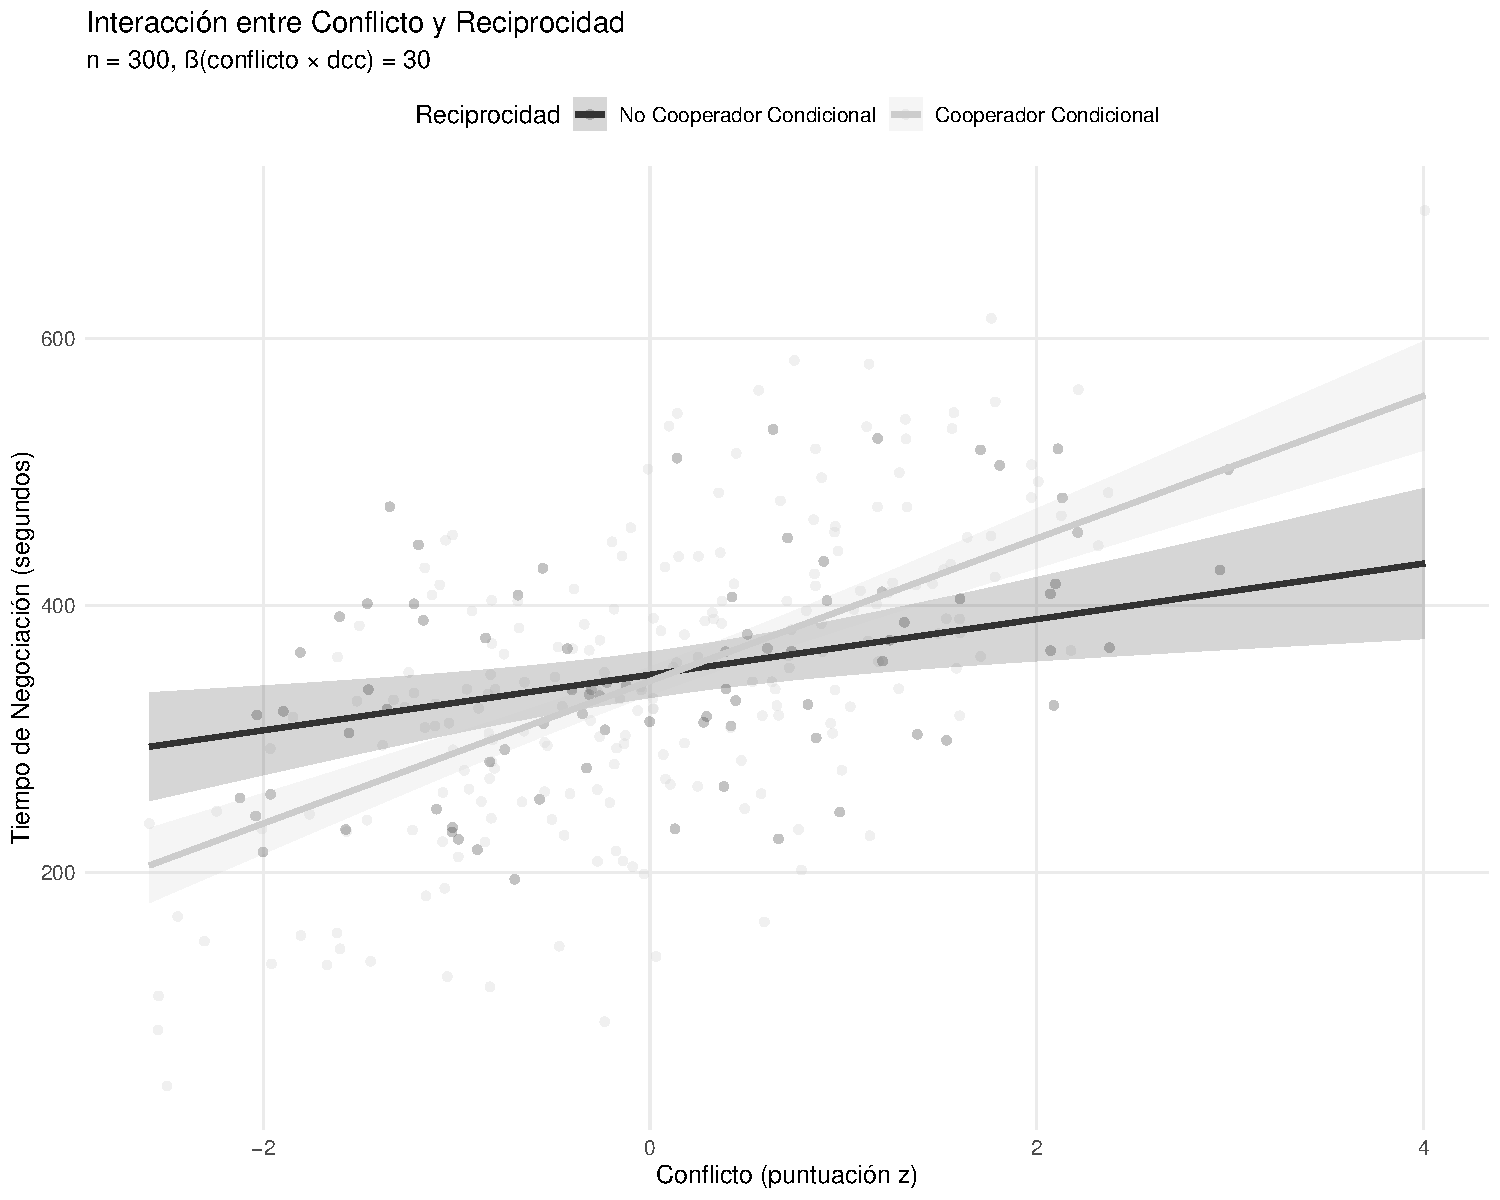
\includegraphics[keepaspectratio]{Prueba1_Amaru_Aguero_files/figure-pdf/fig2-1.pdf}}

}

\caption{Interacción entre conflicto y reciprocidad}

\end{figure}%

\section{Pregunta 7.}\label{pregunta-7.}

Discutir principales resultados y plantear conclusiones del ejercicio y
los modelos.

\section{Repositorio GitHub y
Referencias.}\label{repositorio-github-y-referencias.}

Este
\href{https://github.com/AmaruSimonAgueroJimenez/Econometria-DCCS\%22}{repositorio}
contiene el código fuente de este ejercicio, así como los datos
utilizados para la simulación y análisis. De igual manera se puede
acceder con el siguiente código QR.

\pandocbounded{
\includegraphics[keepaspectratio]{Prueba1_Amaru_Aguero_files/figure-pdf/unnamed-chunk-11-1.pdf}}

El informe .pdf se encuentra en
\href{https://github.com/AmaruSimonAgueroJimenez/Econometria-DCCS/blob/main/docs/Prueba1_Amaru_Aguero.pdf}{esta
dirección}. De igual manera se puede acceder con el siguiente código QR.

\pandocbounded{
\includegraphics[keepaspectratio]{Prueba1_Amaru_Aguero_files/figure-pdf/unnamed-chunk-12-1.pdf}}

\phantomsection\label{refs}
\begin{CSLReferences}{1}{0}
\bibitem[\citeproctext]{ref-gerpott2018how}
1. Gerpott, F. H., Balliet, D., Columbus, S., Molho, C., \& Vries, R. E.
de. (2018). How do people think about interdependence? A
multidimensional model of subjective outcome interdependence.
\emph{Journal of Personality and Social Psychology}, \emph{115}(4),
716-742. \url{https://doi.org/10.1037/pspp0000166}

\bibitem[\citeproctext]{ref-fischbacher2012behavioral}
2. Fischbacher, U., Gächter, S., \& Quercia, S. (2012). The behavioral
validity of the strategy method in public good experiments.
\emph{Journal of Economic Psychology}, \emph{33}(4), 897-913.
\url{https://doi.org/10.1016/j.joep.2012.04.002}

\bibitem[\citeproctext]{ref-murphy2011measuring}
3. Murphy, R. O., Ackermann, K. A., \& Handgraaf, M. J. J. (2011).
Measuring social value orientation. \emph{Judgment and Decision Making},
\emph{6}(8), 771-781. \url{https://ssrn.com/abstract=1804189}

\end{CSLReferences}




\end{document}
